\subsection{Monarch Initiative: Mendelian-disease causality and phenotypic breadth}
\label{sec:monarch}
The GWAS audit (Section~\ref{sec:gwas}) tested common-variant germline
associations of the panel; here we test the complementary rare/Mendelian
axis. We queried the Monarch Initiative knowledge graph v3 (aggregating
OMIM, Orphanet, and HPO annotations) for causal and correlated
gene--disease associations and HPO phenotype annotations of all 205
study genes (204 resolved to HGNC identifiers; the remainder recorded as
unresolved).

\paragraph{Calibration gate.} Pre-registered gates PASSED: (G1) 204/205
genes resolved (threshold 180); (G2) the CD19 sentinel carries at least one
causal gene--disease association (observed 1; OMIM common variable
immunodeficiency 3); (G3) CD19 carries at least ten HPO phenotype
annotations (observed 42). Gate thresholds were calibrated on a
recorded connectivity probe of the live API before the full fetch.

\paragraph{Causality gated versus background.} Genes carrying at least one
causal (Mendelian) disease association: 29/98 gated versus 23/98
background (Fisher odds ratio 1.37, $p=0.419$). Correlated (non-causal)
disease associations: 38/98 versus 26/98 (odds ratio 1.75,
$p=0.0935$). Median HPO phenotypic breadth 0 versus 0
(Mann--Whitney $p=0.856$). Restricting causal associations to disease labels
matching cancer terms: 1/98 gated versus 1/98 ($p=1$).
No Mendelian-causality or phenotypic-breadth axis distinguishes gated antigens from background: the panel's surface antigens are as free of germline Mendelian disease entanglement as the matched background, completing the germline picture alongside the common-variant GWAS null and the somatic-selection constraint audit.

\paragraph{AND-gate antigens.} CA9: no causal disease associations; CA12: 1 causal (isolated hyperchlorhidrosis); CLDN18: no causal disease associations; CLDN6: no causal disease associations; MSLN: no causal disease associations; PSCA: no causal disease associations; SLC39A6: no causal disease associations.

\begin{figure}[t]
\centering
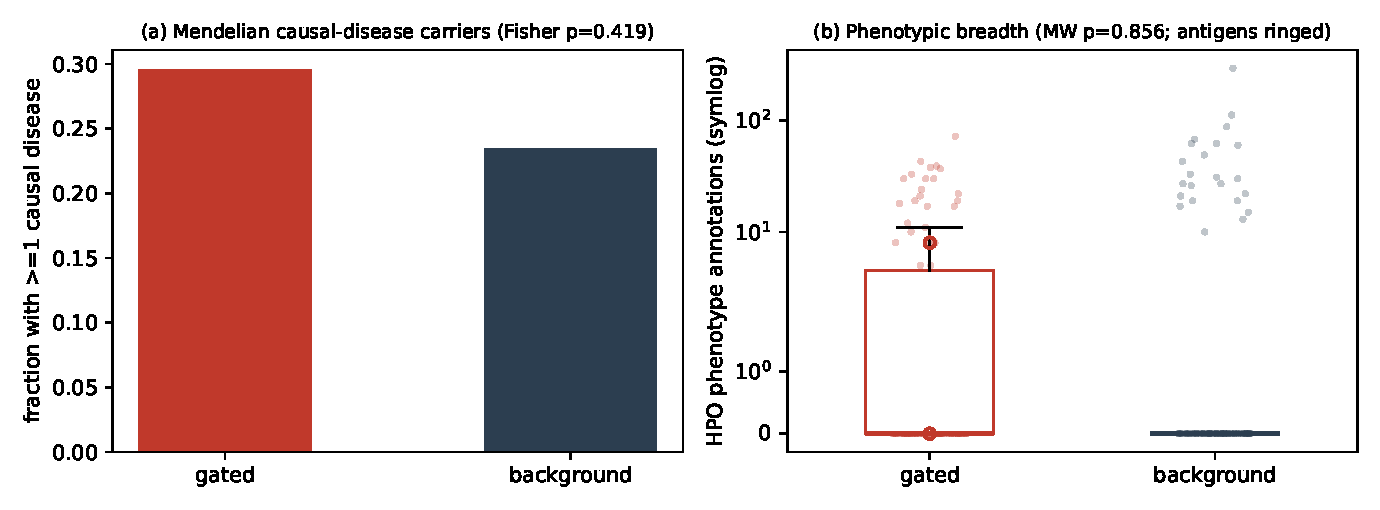
\includegraphics[width=\linewidth]{monarch_fig.pdf}
\caption{Monarch Mendelian-disease and phenotype audit. (a) Fraction of
genes carrying at least one causal gene--disease association. (b) HPO
phenotypic breadth per gene (symlog axis), with the seven AND-gate
antigens ringed.}
\label{fig:monarch}
\end{figure}
